\scanpage{8}
Orientation d'un contour.

Choix pour tte arête $a\in A$ d'une ``orientation de $a$'' i.e. d'une origine $\deleted{\unsure{o|\omega}}\sigma(a)$ de $a$, de telle façon que l'on ait

% slanted
\margin{\diagram{\begin{tikzcd}[ampersand replacement=\&,column sep=small] A \arrow[r,"{\substack{\sigma\\[-.35ex]\sim}}"] \& S \end{tikzcd}}
$\forall a\in A,\ \deleted{\unsure{\exists1|\exists}}(\sigma(a),a)\in R$\\
\deleted{$\unsure{\forall s\in S|\forall a\in S},\exists1\,a\in A,$}}

\[
\begin{aligned}
&\text{Si}\quad \deleted{R\{s\}=\{a,b\},\ \text{alors }\exists}\quad s\in S,\quad \exists1\ a\in R\{s\}\ \text{tel que}\\
&s=\sigma(a).
\end{aligned}\tag*{(\unsure{O|0})}
\]

Réduction au cas connexe

\uline{Prop} Si $(S,A,R)$ est un contour connexe, il a exactement \uline{deux} orientations ($\omega$ et $-\omega$).

\figure{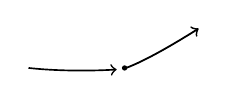
\begin{tikzpicture}[x=.02cm,y=.02cm]
\draw[->,line width=.6pt] (0,0) .. controls (18,-2) and (39,-2) .. (56,-1);
\fill (61,0) circle[radius=1.7];
\draw[->,line width=.65pt] (62,0) .. controls (75,5) and (92,15) .. (108,25);
\end{tikzpicture}}

\figure{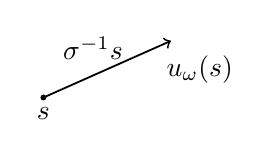
\begin{tikzpicture}[x=.03cm,y=.03cm]
\fill (0,0) circle[radius=1.25];\draw[->,line width=.65pt] (0,0)--(54,24);
\node[below] at (0,0) {$s$};
\node[above] at (21,12) {$\sigma^{-1}s$};
\node[below right] at (48,22) {$u_{\omega}(s)$};
\end{tikzpicture}}
\deleted{Prop} \uline{Prop} Soit $\omega$ orientation du contour $(S,A,R)$.

$\forall s\in S$, soit $\deleted{\unsure{\omega(s)|w(s)}\unsure{u_{\omega}|u}}\inserted{u_{\omega}}(s)$ l'\uline{extrémité} de l'unique arête \inserted{$\sigma^{-1}(s)$} qui ait \deleted{\unsure{comme}} $s$ comme origine
\[
\left[\begin{aligned}(u_{\omega}(s),\sigma^{-1}(s))&\in R,\\u_{\omega}(s)&\ne s\end{aligned}\right]
\]

\figure{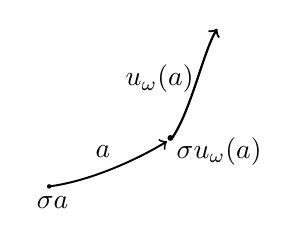
\begin{tikzpicture}[x=.022cm,y=.022cm]
\fill (0,0) circle[radius=1.3];\draw[->,line width=.7pt] (0,0) .. controls (23,3) and (50,15) .. (68,26);
\fill (70,28) circle[radius=1.7];\draw[->,line width=.8pt] (71,28) .. controls (82,44) and (89,78) .. (97,91);
\node[below] at (2,0) {$\sigma a$};\node[above] at (31,11) {$a$};
\node[right] at (68,20) {$\sigma u_{\omega}(a)$};\node[left] at (89,62) {$u_{\omega}(a)$};
\end{tikzpicture}}
$\forall a\in A$, soit $u_{\omega}(a)$ l'unique arc de $S$ dont l'origine soit l'extrémité de $a$
\[
\left[\begin{aligned}
(\sigma u_{\omega}(a),a)&\in R,\quad \sigma u_{\omega}(a)\ne\sigma a\\
&\hspace{6em}\text{i.e.}\quad u_{\omega}(a)\ne a
\end{aligned}\right]
\]

\margin{$\big\}$}Alors $u_{\omega}:(S,\deleted{\unsure{R|B}}A)\unsure{-|\to}(S,A)$ est un autom du graphe $(S,A,R)$. On a $u_{-\omega}=u_{\omega}^{-1}$. Les autom $u_{\omega},u_{\omega}^{-1}$ sont caractérisés par les \deleted{fait que} conditions équivalentes

$1^{\circ})$ $\forall s\in S$, $s$ lié à $gs$

$2^{\circ})$ $\forall a\in A$, $a$ lié à $ga$

Si $n=\operatorname{card}S=\operatorname{card}A$, l'ordre de $u_{\omega},u_{\omega}^{-1}=u_{-\omega}$ est $n$

\unsure{flèche|et} $u_{\omega}\ne u_{-\omega}$ sss $n\ne2$ i.e. $n\geq3$ ; donc $\omega\longmapsto u_{\omega}$ est bijection de $\operatorname{or}(S,A,R)$ avec l'ens des $g\in\operatorname{Aut}(S,A,R)$ satisfaisant les conditions équiv. \unsure{$1^{\circ}$ ou $2^{\circ})\big\}$|$1^{\circ}$ ou $2^{\circ}\big\}$}, Et le \unsure{gpe|grpe} cyclique $\simeq\mathbb{Z}/n\mathbb{Z}$ engendré par $u_{\omega}$ est \deleted{\unsure{formé|form}} \inserted{le} \inserted{gpe $G^{\unsure{0|\circ}}$} des autom \inserted{orientés} de $(S,A,R,\omega)$ \inserted{\unsure{lire|les} de $S,A,R;\omega)$}. $S$ et $A$ sont des \uline{torseurs} sous $G^{0}$.

\deleted{\unsure{Se donner un|La donnée d'un}}

Torseur sous $\mathbb{Z}/n\mathbb{Z}$ \inserted{$(n\geq1)$} $=$ ensemble \deleted{\unsure{où}} à $n$ élément muni d'un ordre $^{\times}$ circulaire. Se donner un contour
% archive sheet number: 7
